\documentclass[12pt,a4paper]{article}
\usepackage{amsmath,amssymb,mathrsfs,tikz,times,pifont}
\usepackage{enumitem}
\usepackage{pgfplots}
\pgfplotsset{compat=1.15}
\usepackage{mathrsfs}
\usetikzlibrary{calc} % Permet de faire des calculs de coordonnées
\usetikzlibrary{arrows}
\pagestyle{empty}
\newcommand\circitem[1]{%
\tikz[baseline=(char.base)]{
\node[circle,draw=gray, fill=red!55,
minimum size=1.2em,inner sep=0] (char) {#1};}}
\newcommand\boxitem[1]{%
\tikz[baseline=(char.base)]{
\node[fill=cyan,
minimum size=1.2em,inner sep=0] (char) {#1};}}
\setlist[enumerate,1]{label=\protect\circitem{\arabic*}}
\setlist[enumerate,2]{label=\protect\boxitem{\alph*}}
%%%::::::by chnini ameur :::::::%%%
\everymath{\displaystyle}
\usepackage[left=1cm,right=1cm,top=1cm,bottom=1.7cm]{geometry}
\usepackage{array,multirow}
\usepackage[most]{tcolorbox}
\usepackage{varwidth}
\tcbuselibrary{skins,hooks}
\usetikzlibrary{patterns}
%%%::::::by chnini ameur :::::::%%%
\newtcolorbox{exa}[2][]{enhanced,breakable,before skip=2mm,after skip=5mm,
colback=yellow!20!white,colframe=black!20!blue,boxrule=0.5mm,
attach boxed title to top left ={xshift=0.6cm,yshift*=1mm-\tcboxedtitleheight},
fonttitle=\bfseries,
title={#2},#1,
% varwidth boxed title*=-3cm,
boxed title style={frame code={
\path[fill=tcbcolback!30!black]
([yshift=-1mm,xshift=-1mm]frame.north west)
arc[start angle=0,end angle=180,radius=1mm]
([yshift=-1mm,xshift=1mm]frame.north east)
arc[start angle=180,end angle=0,radius=1mm];
\path[left color=tcbcolback!60!black,right color = tcbcolback!60!black,
middle color = tcbcolback!80!black]
([xshift=-2mm]frame.north west) -- ([xshift=2mm]frame.north east)
[rounded corners=1mm]-- ([xshift=1mm,yshift=-1mm]frame.north east)
-- (frame.south east) -- (frame.south west)
-- ([xshift=-1mm,yshift=-1mm]frame.north west)
[sharp corners]-- cycle;
},interior engine=empty,
},interior style={top color=yellow!5}}
%%%%%%%%%%%%%%%%%%%%%%%
\usepackage{tkz-tab}
\usepackage{fancyhdr}
\usepackage{eso-pic}         % Pour ajouter des éléments en arrière-plan
% Commande pour ajouter du texte en arrière-plan
\AddToShipoutPicture{
    \AtTextCenter{%
        \makebox[0pt]{\rotatebox{80}{\textcolor[gray]{0.7}{\fontsize{5cm}{5cm}\selectfont PGB}}}
    }
}
\usepackage{lastpage}
% D\'efinition de l'encadr\'e adaptatif avec fond jaune
\newtcolorbox{resultbox}{
    colback=red!30, % Fond rouge clair
    colframe=black, % Bordure noire fine
    sharp corners, % Coins nets
    boxrule=0.5pt, % Contour l\'eger
    boxsep=2pt, % Espacement interne
    left=5pt, right=5pt, top=2pt, bottom=2pt, % Marges internes
}
\fancyhf{}
\pagestyle{fancy}
\renewcommand{\footrulewidth}{1pt}
\renewcommand{\headrulewidth}{0pt}
\renewcommand{\footruleskip}{10pt}
\fancyfoot[R]{
\color{blue}\ding{45}\ \textbf{2025}
}
\fancyfoot[L]{
\color{blue}\ding{45}\ \textbf{Prof:M. BA}
}
\cfoot{\bf
\thepage/\pageref{LastPage}}
\begin{document}
\renewcommand{\arraystretch}{1.5}
\renewcommand{\arrayrulewidth}{1.2pt}
\begin{tikzpicture}[overlay,remember picture]
    \node[draw=blue,line width=1.2pt,fill=purple,text=blue,inner sep=3mm,rounded corners,pattern=dots]at ([yshift=-2.5cm]current page.north) {\begingroup\setlength{\fboxsep}{0pt}\colorbox{white}{\begin{tabular}{|*1{>{\centering \arraybackslash}p{0.28\textwidth}} |*2{>{\centering \arraybackslash}p{0.2\textwidth}|} *1{>{\centering \arraybackslash}p{0.19\textwidth}|} }
                \hline
                \multicolumn{3}{|c|}{$\diamond$$\diamond$$\diamond$\ \textbf{Lycée de Dindéfélo}\ $\diamond$$\diamond$$\diamond$ } & \textbf{A.S. : 2024/2025}                                                                     \\ \hline
                \textbf{Matière: Mathématiques}                                                                                    & \textbf{Niveau : 1}\textbf{$^{er}$S2} & \textbf{Date: 19/03/2025} & \textbf{Durée : 4 heures} \\ \hline
                \multicolumn{4}{|c|}{\parbox[c]{10cm}{\begin{center}
                                                                  \textbf{{\Large\sffamily Devoir n$ ^{\circ} $ 1 Du 2$ ^\text{\bf nd} $ Semestre}}
                                                              \end{center}}}                                                                                                                               \\ \hline
            \end{tabular}}\endgroup};
\end{tikzpicture}
\vspace{3cm}

\section*{\underline{Exercice 1 :} 5 pts }
Déterminons le domaine de définition dans chaque cas
\begin{enumerate}
    \item $f(x) = \sqrt{4x - x^3}$

\( f\quad \exists\quad  \text{ ssi } \quad 4x - x^3 \geq 0 \)

Posons \( 4x - x^3 = 0 \)

\(
\begin{aligned}
4x - x^3 = 0 &\implies x(4 - x^2) = 0\\
						 &\implies x = 0 \textbf{ ou } 4 - x^2 = 0\\
 						 &\implies	x = 0 \textbf{ ou } x = 2 \textbf{ ou } x = -2
\end{aligned}
\)  

\begin{center}
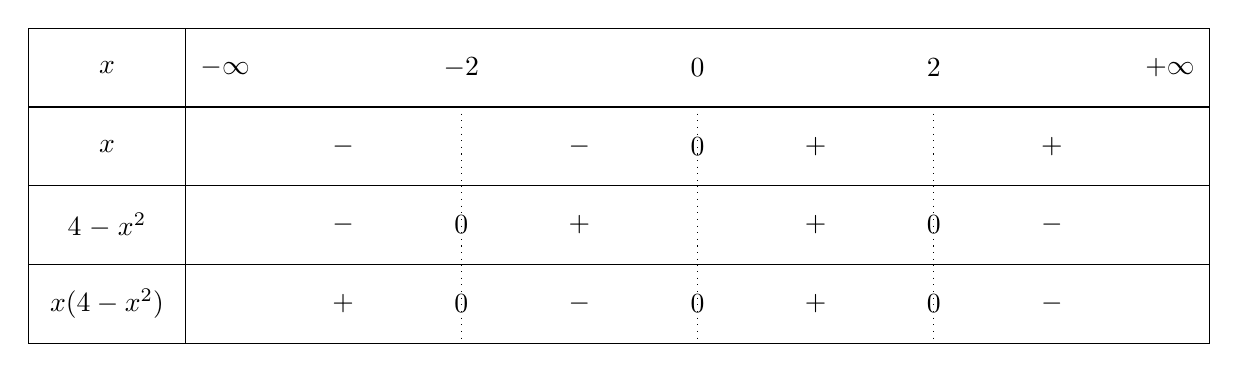
\begin{tikzpicture}
    % Création du tableau
    \tkzTabInit{$x$ / 1 , $x$ / 1 , $4 - x^2$ / 1 , $x(4 - x^2)$ / 1}
      { $-\infty$, $-2$, $0$, $2$, $+\infty$ }
    % Ligne x+1
    \tkzTabLine{ , - , t , - , z ,+, t ,+, }
    % Ligne 2x+3
    \tkzTabLine{ , - , z , + , t ,+,z ,-, }
    % Ligne P(x)
    \tkzTabLine{ , + , z , - , z ,+, z,-, }
\end{tikzpicture}
\end{center}    

\begin{center}
\( Df = ]-\infty;-2] \cup [0 ; 2 ] \) 
\end{center}   

          \begin{resultbox}
            \[
                \mathbf{Df = ]-\infty;-2] \cup [0 ; 2 ]\quad\quad\quad \textbf{1pt}}
            \]
        \end{resultbox}     
    
    \item $f(x) = \sqrt{|1 - 3x| - x + 2}$
    
    \( f\quad \exists\quad  \text{ ssi } \quad |1 - 3x| - x + 2 \geq 0 \)

\(
\begin{aligned}
|1 - 3x| - x + 2 \geq 0 &\implies |1 - 3x| \geq  x - 2\\
						 &\implies 1 - 3x \geq  x - 2 \textbf{ ou } 1 - 3x \leq  -x + 2\\
 						 &\implies	4x \leq 3 \textbf{ ou }  2x \geq  -1\\
 						 &\implies	x \leq \frac{3}{4} \textbf{ ou }  x \geq \frac{-1}{2}\\
\end{aligned}
\)  

\(    
\begin{aligned}
Df &= \left]-\infty;\frac{3}{4}\right] \cup \left[\frac{-1}{2} ; +\infty\right[\\ 
&= \left]-\infty ; +\infty\right[ \\
&=\mathbb{R}
\end{aligned}
\)

          \begin{resultbox}
            \[
                \mathbf{Df = \mathbb{R}\quad\quad\quad \textbf{1pt}}
            \]
        \end{resultbox} 

    \item $\left\{
        \begin{array}{ll}
            f(x) = x \sqrt{\left| \dfrac{x+1}{x} \right|}, & \text{si } x < 0 \\
            f(x) = \dfrac{x^3 - x^2}{x^2 + 1}, & \text{si } x \geq 0
        \end{array}
    \right.$

Posons$\left\{
        \begin{array}{ll}
            f_{1}(x) = x \sqrt{\left| \dfrac{x+1}{x} \right|}, & \text{si } x < 0 \\
            f_{2}(x) = \dfrac{x^3 - x^2}{x^2 + 1}, & \text{si } x \geq 0
        \end{array}
    \right.$    

\( f_{1}\quad \exists \text{ ssi } \quad  \left| \dfrac{x+1}{x} \right| \geq 0 \text{ et } x \neq 0 \text{ et } x < 0\)    

\( Df_{1} = \left]-\infty;0\right[ \)

\( f_{2}\quad \exists \text{ ssi } \quad  x^2 + 1 \neq 0 \text{ et } x \geq 0\)    

\( Df_{2} = \left[0;+\infty\right[ \)

\begin{center}
\( Df=Df_{1} \cup Df_{2} \)\\
\( Df=\left]-\infty;0\right[ \cup \left[0;+\infty\right[ \)\\
\( Df=\mathbb{R} \)
\end{center}    

              \begin{resultbox}
            \[
                \mathbf{Df = \mathbb{R}\quad\quad\quad \textbf{1pt}}
            \]
        \end{resultbox} 
    \item $\left\{
        \begin{array}{ll}
            f(x) = \dfrac{x(x-2)}{x-1}, & \text{si } x < 0 \\
            f(x) = x + \sqrt{x^2 - 4}, & \text{si } x \geq 0
        \end{array}
    \right.$

Posons$\left\{
        \begin{array}{ll}
            f_{1}(x) = \dfrac{x(x-2)}{x-1}, & \text{si } x < 0 \\
            f_{2}(x) = x + \sqrt{x^2 - 4}, & \text{si } x \geq 0
        \end{array}
    \right.$    

\( f_{1}\quad \exists \text{ ssi } \quad  x-1 \neq 0  \text{ et } x < 0\)   

\( x-1 \neq 0  \text{ et } x < 0 \)    

\(   x\neq 1  \text{ et } x < 0 \)     

\(   x\neq 1 \text{ et } x\in ]-\infty;0[ \)     

\(   x\in ]-\infty;0[ \)    

\( x\in ]-\infty;0[ \)
    
\( Df_{1}=]-\infty;0[ \)

\( f_{2}\quad \exists \text{ ssi } \quad  x^2 - 4 \geq 0  \text{ et } x \geq 0\)   

Posons \( f_{2}\quad \exists \text{ ssi } \quad  x^2 - 4 = 0  \text{ et } x = 0\)   

\begin{center}
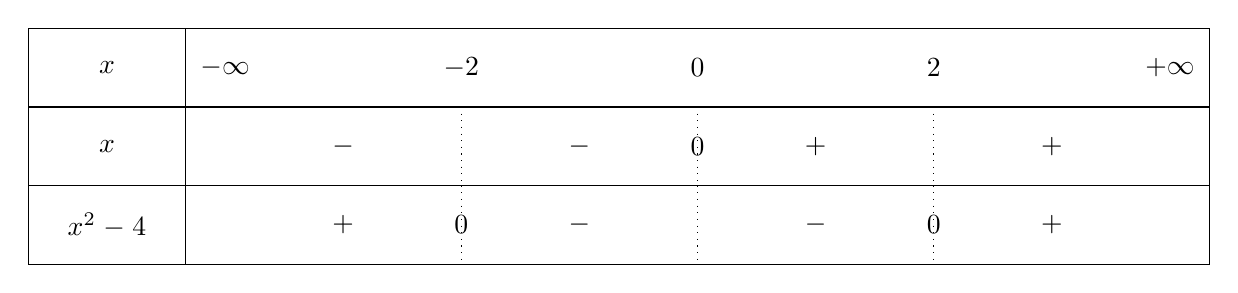
\begin{tikzpicture}
    % Création du tableau
    \tkzTabInit{$x$ / 1 , $x$ / 1 , $x^2-4$ / 1}
      { $-\infty$, $-2$, $0$, $2$, $+\infty$ }
    % Ligne x+1
    \tkzTabLine{ , - , t , - , z ,+, t ,+, }
    % Ligne 2x+3
    \tkzTabLine{ , + , z , - , t ,-,z ,+, }
\end{tikzpicture}
\end{center}

\( Df_{2}=[2;+\infty[ \)

\begin{center}
\( Df=Df_{1} \cup Df_{2} \)\\
\( Df=]-\infty;0[ \cup [2;+\infty[ \)
\end{center}    

              \begin{resultbox}
            \[
                \mathbf{Df = ]-\infty;0[ \cup [2;+\infty[ \quad\quad\quad \textbf{1pt}}
            \]
        \end{resultbox} 
    \item $\left\{
        \begin{array}{ll}
            f(x) = \dfrac{3}{|x+1| - 2}, & \text{si } x \leq 1 \\
            f(x) = \sqrt{x - 3}, & \text{si } x > 1
        \end{array}
    \right.$
    
Posons  $\left\{
        \begin{array}{ll}
            f_{1}(x) = \dfrac{3}{|x+1| - 2}, & \text{si } x \leq 1 \\
            f_{2}(x) = \sqrt{x - 3}, & \text{si } x > 1
        \end{array}
    \right.$
    
\( 
\begin{array}{llll}
            f_{1}\quad \exists \text{ ssi }& \quad  |x+1| - 2 \neq 0 & \text{ et } & x \leq 1 \\
       			 																&\quad  |x+1|  \neq 2 & \text{ et } & x \leq 1 \\
       																			&\quad  x+1  \neq -2\text{ ou } x+1  \neq 2 & \text{ et } & x \leq 1 \\
       																			&\quad  x \neq -3\text{ ou } x \neq 1 & \text{ et } & x \leq 1 \\
       																			&\quad  x \neq -3\text{ ou } x \neq 1 & \text{ et } & x \in ]-\infty;1] \\
       																			&\quad x \in ]-\infty;-3[\cup]-3;1[\\
        \end{array} \\
\) 

\begin{center}
\( Df_{1} = ]-\infty;-3[\cup]-3;1[ \)\\
\end{center}     

\( 
\begin{array}{llll}
            f_{2}\quad \exists \text{ ssi }& \quad  x - 3 \geq 0 & \text{ et } & x > 1 \\
       			 																& \quad  x  \geq 3 & \text{ et } & x > 1 \\
       																			& \quad  x\in [3;+\infty[ & \text{ et } & x\in ]1;+\infty[\\
       																			& \quad  x \in ]1;+\infty[ & \cap & x \in[3;+\infty[\\
       																			& \quad  x \in ( ]1;+\infty[ & \cap &  [3;+\infty[)\\
       																			& \quad x \in [3;+\infty[
        \end{array} \\
\) 

\begin{center}
\( Df_{2} = [3;+\infty[ \)\\
\end{center}     

\begin{center}
\( Df=Df_{1} \cup Df_{2} \)\\
\( Df=(]-\infty;-3[\cup]-3;1[)\cup[3;+\infty[ \)
\end{center} 

              \begin{resultbox}
            \[
                \mathbf{Df = \left( ]-\infty;-3[\cup]-3;1[\right) \cup[3;+\infty[ \quad\quad\quad \textbf{1pt}}
            \]
        \end{resultbox}     
    
\end{enumerate}

\section*{\underline{Exercice 2 :} 4 pts }

\begin{enumerate}
    \item Dans chacun des cas suivants, montrons que \( (C_f) \) admet la droite \( (\Delta) \) pour axe de symétrie.

\begin{enumerate}
    \item \( f(x) = -3x^2 + 4x + 1 \) et \( (\Delta) : x = \frac{2}{3} \).
    
    \( (\Delta) : x = \frac{2}{3} \) est axe de symétrie ssi \( f(2a - x) = f(x) \) où \( a = \frac{2}{3} \)
    
    \(
    \begin{aligned}
    	f(2a - x) = f(x)  & \implies -3(2a - x)^2 + 4(2a - x) + 1 = -3x^2 + 4x + 1 \\
    										& \implies -3\left( 2\times\frac{2}{3} - x\right) ^2 + 4\left( 2\times\frac{2}{3} - x\right)  + 1 = -3x^2 + 4x + 1 \\
    										& \implies -3\left( \frac{4}{3} - x\right) ^2 + 4\left( \frac{4}{3} - x\right)  + 1 = -3x^2 + 4x + 1 \\
    										& \implies -3\left( \frac{16}{9} + x^{2} - \frac{8x}{3}\right) + \left( \frac{16}{3} - 4x\right)  + 1 = -3x^2 + 4x + 1 \\
    										& \implies \frac{-16}{3} - 3x^{2} + 8x +  \frac{16}{3} - 4x  + 1 = -3x^2 + 4x + 1 \\
    										& \implies - 3x^{2} + 4x  + 1 = -3x^2 + 4x + 1 \textbf{ vrai }\\
    										&\text{ Donc \(  x = \frac{2}{3} \) est bien axe de symétrie }
    \end{aligned}
    \)

          \begin{resultbox}
            \[
                \mathbf{\text{ Donc \(  x = \frac{2}{3} \) est bien axe de symétrie }\quad\quad\quad \textbf{0,75pt}}
            \]
        \end{resultbox}    
    
    \item \( f(x) = \frac{x^2 + 4x + 3}{2x^2 + 8x + 9} \) et \( (\Delta) : x = -2 \).
    
    \( (\Delta) : x = -2 \) est axe de symétrie ssi \( f(2a - x) = f(x) \) où \( a =  -2 \)
    
    \(
    \begin{aligned}
    	f(2a - x) = f(x)  & \implies \frac{(2a - x)^2 + 4(2a - x) + 3}{2(2a - x)^2 + 8(2a - x) + 9} = \frac{x^2 + 4x + 3}{2x^2 + 8x + 9} \\
    										& \implies \frac{(2\times(-2) - x)^2 + 4(2\times(-2) - x) + 3}{2(2\times(-2) - x)^2 + 8(2\times(-2) - x) + 9} = \frac{x^2 + 4x + 3}{2x^2 + 8x + 9} \\
    										& \implies \frac{(-4 - x)^2 + 4(-4 - x) + 3}{2(-4 - x)^2 + 8(-4 - x) + 9} = \frac{x^2 + 4x + 3}{2x^2 + 8x + 9} \\
    										& \implies \frac{16 + 8x + x^2 -16-4x + 3}{2(16 + 8x + x^2) -32-8x + 9} = \frac{x^2 + 4x + 3}{2x^2 + 8x + 9} \\
    										& \implies \frac{x^2 + 4x + 3}{32 + 16x + 2x^2 -32-8x + 9} = \frac{x^2 + 4x + 3}{2x^2 + 8x + 9} \\
    										& \implies \frac{x^2 + 4x + 3}{2x^2+8x + 9} = \frac{x^2 + 4x + 3}{2x^2 + 8x + 9}\textbf{ vrai } \\
    										&\text{ Donc \(  x = -2 \) est bien axe de symétrie }
    \end{aligned}
    \)

          \begin{resultbox}
            \[
                \mathbf{\text{ Donc \(  x = -2 \) est bien axe de symétrie }\quad\quad\quad \textbf{0,75pt} }
            \]
        \end{resultbox}    
    
\end{enumerate}
\item  Dans chacun des cas suivants, montrons que \( (C_f) \) admet le point \( I \) pour centre de symétrie.

\begin{enumerate}
    \item \( f(x) = -x^3 + 3x + 4 \) et \( I(0;4) \).
    
    \( I(0;4) \) est centre de symétrie ssi \( f(2a - x) + f(x) = 2 \times b \)  où \( a =  0 \text{ et } b = 4 \)
    
        \(
    \begin{aligned}
    	f(2a - x) + f(x) = 2 \times b  & \implies -(2a - x)^3 + 3(2a - x) + 4 + -x^3 + 3x + 4 = 2 \times b\\
    																 & \implies -(2\times 0 - x)^3 + 3(2\times 0 - x) + 4 + -x^3 + 3x + 4 = 2 \times4\\
    																 & \implies x^3 -3x + 4 -x^3 + 3x + 4 = 8\\
    																 & \implies 8 = 8\textbf{ vrai }\\
    										&\text{ Donc \( I(1;1) \) est bien centre de symétrie }
    \end{aligned}
    \)

          \begin{resultbox}
            \[
                \mathbf{\text{ Donc \( I(1;1) \) est bien centre de symétrie } \quad\quad\quad \textbf{0,75pt}}
            \]
        \end{resultbox}    
    
    \item \( f(x) = \frac{x^3 - x^2 - x}{2x^2 - 4x + 1} \) et \( I(1;1) \).

\( I(1;1) \) est centre de symétrie ssi \( f(2a - x) + f(x) = 2 \times b \)  où \( a =  1 \text{ et } b = 1 \)
    
        \(
    \begin{aligned}
    	f(2a - x) + f(x) = 2 \times b  & \implies \frac{(2a - x)^3 - (2a - x)^2 - (2a - x)}{2(2a - x)^2 - 4(2a - x) + 1} + \frac{x^3 - x^2 - x}{2x^2 - 4x + 1} = 2 \times b\\
    	& \implies \frac{(2 - x)^3 - (2 - x)^2 - (2 - x)}{2(2 - x)^2 - 4(2 - x) + 1} + \frac{x^3 - x^2 - x}{2x^2 - 4x + 1} = 2 \times 1\\
    	    	& \implies \frac{8 -12x+6x^{2}-x^{3} - (4 - 4x + x^{2}) - 2 + x}{2(4 -4x + x^{2}) - 4(2 - x) + 1} + \frac{x^3 - x^2 - x}{2x^2 - 4x + 1} = 2 \times 1\\
    	    	& \implies \frac{8 -12x+6x^{2}-x^{3} - 4 + 4x - x^{2} - 2 + x}{2(4 -4x + x^{2}) - 4(2 - x) + 1} + \frac{x^3 - x^2 - x}{2x^2 - 4x + 1} = 2 \times 1\\
    	    	& \implies \frac{8 -12x+6x^{2}-x^{3} - 4 + 4x - x^{2} - 2 + x}{8 -8x + 2x^{2} - 8 + 4x + 1} + \frac{x^3 - x^2 - x}{2x^2 - 4x + 1} = 2 \times 1\\
    	    	& \implies \frac{-x^{3} + 5x^{2} - 7x +2 }{2x^{2} - 4x + 1} + \frac{x^3 - x^2 - x}{2x^2 - 4x + 1} = 2 \times 1\\
    	    	& \implies \frac{ -x^3+5x^{2} - 7x +2+ x^3 - x^2 - x}{2x^{2} - 4x + 1} = 2 \times 1\\
    	    	& \implies \frac{ 4x^{2} - 8x +2 }{2x^{2} - 4x + 1} = 2 \times 1\\
    	    	& \implies \frac{ 2(2x^{2} - 4x +1) }{2x^{2} - 4x + 1} = 2 \times 1\\
    	    	& \implies 2\times 1 = 2 \times 1\\
    																 & \implies 2 = 2\textbf{ vrai }\\
    										&\text{ Donc \( I(0;4) \) est bien centre de symétrie }
    \end{aligned}
    \)

          \begin{resultbox}
            \[
                \mathbf{\text{ Donc \( I(0;4) \) est bien centre de symétrie } \quad\quad\quad \textbf{0,75pt}}
            \]
        \end{resultbox}    
    
    \newpage
    \item \( f(x) = \frac{1}{x+3} + \frac{1}{x+1} \) et \( I(-2;0) \).
    
    \( I(-2;0) \) est centre de symétrie ssi \( f(2a - x) + f(x) = 2 \times 0 \)  où \( a =  -2 \text{ et } b = 0 \)
    
\(
\begin{aligned}
    	f(2a - x) + f(x) = 2 \times b  & \implies \frac{1}{(2a - x)+3} + \frac{1}{(2a - x)+1} + \frac{1}{x+3} + \frac{1}{x+1}= 2 \times 0\\
    																 & \implies \frac{1}{(2\times (-2) - x)+3} + \frac{1}{(2\times (-2) - x)+1}+ \frac{1}{x+3} + \frac{1}{x+1} = 2 \times 0\\     	
    																 & \implies \frac{1}{-4 - x+3} + \frac{1}{-4 - x+1} + \frac{1}{x+3} + \frac{1}{x+1} = 2 \times 0\\
    																 & \implies -\frac{1}{  x + 1} - \frac{1}{ x + 3} + \frac{1}{x+3} + \frac{1}{x+1}= 2 \times 0\\
    																 & \implies 0 = 0\textbf{ vrai }\\
    										&\text{ Donc \( I(-2;0) \) est bien centre de symétrie }
\end{aligned}
\)

          \begin{resultbox}
            \[
                \mathbf{\text{ Donc \( I(-2;0) \) est bien centre de symétrie } \quad\quad\quad \textbf{1pt}}
            \]
        \end{resultbox}
\end{enumerate}

\end{enumerate}

\section*{\underline{Exercice 3:} 5pts }

\begin{enumerate}
\item Soient les fonctions \( f \) et \( g \) telles que :

$
    \begin{aligned}
        f : \mathbb{R} & \to \mathbb{R} \\
        x              & \mapsto x^2
    \end{aligned}\quad\quad\quad
    \begin{aligned}
        g : \mathbb{R} & \to \mathbb{R}        \\
        x              & \mapsto 2x^2 - 5x - 3
    \end{aligned}
$
\begin{enumerate}
    \item Montrons que \( f \) et \( g \) sont des applications. \hfill \textbf{(0,5 pt)}

          \( Df=\mathbb{R} \) donc \(f\) est une application

          \( Dg=\mathbb{R} \) donc \(g\) est une application
    \item Les fonctions \( f \) et \( g \) sont-elles injectives ? Surjectives ? \hfill
          \textbf{(2 $\times$ 0,5 pt)}

          \underline{\textbf{Pour \( f \)}}:

            Vérifions si \( f \) injective

          Soit \(x_1\) et \(x_2\) \(\in \mathbb{R}\) a-t-on \(f(x_1)=f(x_2)\implies
          x_1=x_2\)?

          \(\begin{aligned}
              f(x_1)=f(x_2) & \implies x_1^{2}=x_2^{2}              \\
                            & \implies x_1=x_2 \text{ ou } x_1=-x_2
          \end{aligned}\)

          \begin{resultbox}
            \[
                \mathbf{\text{Donc \(f\) n'est pas injective}}
            \]
        \end{resultbox}

          Vérifions si \( f \) surjective

          Soit \(y \in \mathbb{R}\) a-t-on \(\forall x \in \mathbb{R},f(x)=y \)?

          \(
          \begin{aligned}
              f(x)=y & \implies x^{2}=y \\
                     & \implies x^{2}=y
          \end{aligned}
          \)

          Cette équation n'a pas toujours une solution. Car si \( y<0 \) alors pas de
          solution.

          \begin{resultbox}
            \[
                \mathbf{\text{Donc \( f \) n'est pas surjective non plus.}}
            \]
        \end{resultbox}
          
          \underline{\textbf{Pour \( g \)}}:
          
          Vérifions si \( g \) injective

          Soit \(x_1\) et \(x_2\) \(\in \mathbb{R}\) a-t-on \(g(x_1)=g(x_2)\implies
          x_1=x_2\)?

          \(\begin{aligned}
              g(x_1)=g(x_2) & \implies 2x_1^{2}-5x_1-3=2x_2^{2}-5x_2-3\\
                            & \implies 2x_1^{2}-5x_1=2x_2^{2}-5x_2\\
                            & \implies 2x_1^{2}-2x_2^{2}-5x_1+5x_2 = 0\\
                            & \implies 2[x_1^{2}-x_2^{2}]-5(x_1-x_2) = 0\\
                            & \implies 2[(x_1-x_2)(x_1+x_2)]-5(x_1-x_2) = 0\\
                            & \implies (x_1-x_2)[2(x_1+x_2)-5] = 0\\
                            & \implies (x_1-x_2)=0 \text{ ou } [2(x_1+x_2)-5] = 0\\
                            & \implies x_1=x_2\text{ ou } 2x_1 = -2x_2+5\\
          \end{aligned}\)

          \begin{resultbox}
            \[
                \mathbf{\text{Donc \(g\) n'est pas injective}}
            \]
        \end{resultbox}

        Vérifions si \( g \) surjective

          Soit \(y \in \mathbb{R}\) a-t-on \(\forall x \in \mathbb{R},g(x)=y \)?

          \(
          \begin{aligned}
              g(x)=y & \implies 2x^{2}-5x-3=y \\
                     & \implies 2x^{2}-5x-3-y=0\\
          \end{aligned}
          \)

            \(
            \begin{aligned}
                \Delta &= 5^{2}-4(2)(-3-y)\\
                       &= 25-8(-3-y)\\
                       &= 25+24+8y\\
                       &= 49+8y\\
            \end{aligned} 
            \)

            Si $y\in \left]-\infty;\frac{-49}{8}\right[$ alors il n'existe pas de $x\in\mathbb{R}$ tel que $g(x)=y$

          \begin{resultbox}
            \[
                \mathbf{\text{Donc \( g \) n'est pas surjective non plus.}}
            \]
        \end{resultbox}

        \end{enumerate}

   \item Soit l’application 

$    
\begin{aligned}
        h : ]3 ; +\infty[ &\to ]0 ; +\infty[ \\
        x &\mapsto 2x^2 - 5x - 3
\end{aligned}
$

   Démontrons que \( h \) est une bijection.

   Soit \(y \in \mathbb{R}\) montrons \(\forall x \in \mathbb{R},g(x)=y \)

          \(
          \begin{aligned}
              g(x)=y & \implies 2x^{2}-5x-3=y \\
                     & \implies 2x^{2}-5x-3-y=0\\
          \end{aligned}
          \)

            \(
            \begin{aligned}
                \Delta &= 5^{2}-4(2)(-3-y)\\
                       &= 25-8(-3-y)\\
                       &= 25+24+8y\\
                       &= 49+8y\\
            \end{aligned} 
            \)

            Comme $y>0$ donc $ \Delta > 0 $ donc $\forall x \in ]3;+\infty[$, $\exists y\in ]0;+\infty[$ tel que $ h(x)=y $ 

          \begin{resultbox}
            \[
                \mathbf{\text{Donc \( h \) est surjective.}}
            \]
        \end{resultbox}
   
   Déterminons sa bijection réciproque \( h^{-1} \). \hfill \textbf{(1 pt)}

   Comme \( \Delta = 49+8y \) donc \( x_{1} = \frac{5-\sqrt{49+8y}}{4} \) et \( x_{2} = \frac{5+\sqrt{49+8y}}{4} \) 

   Or \(\forall y \in ]0;+\infty[ \), \( 49+8y > 5 \) donc \( x_{1}<0 \) et \( x_{2}>0 \)

   Donc \( h^{-1}(x) = \frac{5+\sqrt{49+8x}}{4} \)
   
   \( Dh^{-1}=\left[\frac{-49}{8};+\infty\right[\)

   \begin{resultbox}
    \[
        \mathbf{ h^{-1}(x) = \frac{5+\sqrt{49+8x}}{4} }
    \]
    \end{resultbox}

   \item On considère les intervalles \( I = [4 ; 5] \) et \( J = [0 ; 4] \).
\end{enumerate}

Déterminons l’image directe de $I$ par $h$ et l’image réciproque de $J$ par $h$.\hfill \textbf{(2x0,5 pt)}

\textbf{Calculons h(I)}

\( 
\begin{aligned}
    \forall x \in Dh \cap [4 ; 5] &\implies x \in [4 ; 5] \\
                                &\implies 4 \leq x \leq 5 \\
                                &\implies 16 \leq 2x^{2} \leq 25 \\
                                &\implies 32 \leq 2x^{2} \leq 50 \\
\end{aligned} 
\) 

\( 
\begin{aligned}
    \forall x \in Dh \cap [4 ; 5] &\implies x \in [4 ; 5] \\
                                &\implies 4 \leq x \leq 5 \\
                                &\implies -20 \leq -5x \leq -25 \\
                                &\implies -23 \leq -5x -3 \leq -28 \\
\end{aligned} 
\) 


\underline{\( 
\begin{cases}
    32 \leq 2x^{2} \leq 50 \\
    -23 \leq -5x -3 \leq -28 
\end{cases}
\)}

\( 9 \leq 2x^{2}-5x -3 \leq 22  \)

Donc \( \forall x\in [4;5], 9 \leq x \leq 22  \implies h([4;5]) = [ 9 ; 22] \)

Finalement \( h([4 ; 5]) = [ 9 ; 22] \)

\textbf{Calculons }\( h^{-1}(J) \)

$    
\begin{aligned}
        h^{-1} : ]0 ; +\infty[ &\to ]3 ; +\infty[ \\
        x &\mapsto \frac{5+\sqrt{49+8x}}{4}
\end{aligned}
$

 \( Dh^{-1}=\left[\frac{-49}{8};+\infty\right[\)

\( 
\begin{aligned}
    \forall x \in Dh^{-1} \cap [0 ; 4] &\implies x \in [0; 4] \\
                                &\implies 0 \leq h^{-1}(x) \leq 4 \\
                                &\implies 0 \leq \frac{5+\sqrt{49+8x}}{4} \leq 4 \\
                                &\implies 0 \leq 5+\sqrt{49+8x} \leq 16 \\
                                &\implies -5 \leq \sqrt{49+8x} \leq 11 \\
                                &\implies 25 \leq 49+8x \leq 121 \\
                                &\implies 25-49 \leq 8x \leq 121-49 \\
                                &\implies -24 \leq 8x \leq 72 \\
                                &\implies -3 \leq x \leq 9 \\
                                &\implies h^{-1}(x)\in[-3 ; 9] \\
\end{aligned} 
\) 

Donc \( \forall x\in [0;4], -3 \leq x \leq 9  \implies h^{-1}([0;4]) = [ -3 ; 9] \)

Finalement \( h^{-1}([0;4]) = [ -3 ; 9] \)

\section*{\underline{Exercice 4 :} 6 pts }
Dans le plan, on considère le triangle \( ABC \) tel que \( AB = 2 \), \( AC = 4\sqrt{2} \) et \( BC = 2\sqrt{5} \) (unité cm).
\( I \) est le milieu de \( [AB] \).

\begin{enumerate}
    \item
          \begin{enumerate}
              \item Calculons \( \overrightarrow{AB} \cdot \overrightarrow{AC} \). \hfill
                    \textbf{(01 pt)}

                    \(
                    \begin{aligned}
                        \overrightarrow{BC}=\overrightarrow{BA}+\overrightarrow{AC} & \implies \overrightarrow{BC}^{2}=(\overrightarrow{BA}+\overrightarrow{AC})^{2}                                                                    \\
                                                                                    & \implies \overrightarrow{BC}^{2}=\overrightarrow{BA}^{2}+\overrightarrow{AC}^{2}+2\overrightarrow{BA}.\overrightarrow{AC}                         \\
                                                                                    & \implies \overrightarrow{BC}^{2}=\overrightarrow{BA}^{2}+\overrightarrow{AC}^{2}-2\overrightarrow{AB}.\overrightarrow{AC}                         \\
                                                                                    & \implies 2\overrightarrow{AB}.\overrightarrow{AC}=\overrightarrow{BA}^{2}+\overrightarrow{AC}^{2}-\overrightarrow{BC}^{2}                         \\
                                                                                    & \implies \overrightarrow{AB}.\overrightarrow{AC}=\frac{1}{2}\left( \overrightarrow{BA}^{2}+\overrightarrow{AC}^{2}-\overrightarrow{BC}^{2}\right) \\
                    \end{aligned}
                    \)

                    \begin{resultbox}
                        \[
                            \mathbf{\overrightarrow{AB}.\overrightarrow{AC}=\frac{1}{2}\left( \overrightarrow{BA}^{2}+\overrightarrow{AC}^{2}-\overrightarrow{BC}^{2}\right)}
                        \]
                    \end{resultbox}

                    \(
                    \begin{aligned}
                        \overrightarrow{AB}.\overrightarrow{AC} & =\frac{1}{2}\left( 2^{2}+(4\sqrt{2})^{2}-(2\sqrt{5})^{2}\right) \\
                        \overrightarrow{AB}.\overrightarrow{AC} & =\frac{1}{2}\left( 4+32-20\right)                               \\
                        \overrightarrow{AB}.\overrightarrow{AC} & =\frac{1}{2}\left( 36-20\right)                                 \\
                        \overrightarrow{AB}.\overrightarrow{AC} & =\frac{1}{2}\left( 16\right)                                    \\
                        \overrightarrow{AB}.\overrightarrow{AC} & =8
                    \end{aligned}
                    \)

                    \begin{resultbox}
                        \[
                            \mathbf{\overrightarrow{AB}.\overrightarrow{AC}=8}
                        \]
                    \end{resultbox}

              \item Déduisons-en \( \cos \widehat{BAC} \).\hfill \textbf{(0,5 pt)}

                    \(
                    \begin{aligned}
                        \overrightarrow{AB}.\overrightarrow{AC}= AB\times AC \times \cos \widehat{BAC} & \implies \cos \widehat{BAC}=\frac{\overrightarrow{AB}.\overrightarrow{AC}}{AB\times AC} \\
                                                                                                       & \implies \cos \widehat{BAC}=\frac{8}{2\times 4\sqrt{2}}                                 \\
                                                                                                       & \implies \cos \widehat{BAC}=\frac{1}{\sqrt{2}}                                          \\
                                                                                                       & \implies \cos \widehat{BAC}=\frac{\sqrt{2}}{2}                                          \\
                    \end{aligned}
                    \)

                    \begin{resultbox}
                        \[
                            \mathbf{\cos \widehat{BAC}=\frac{\sqrt{2}}{2}}
                        \]
                    \end{resultbox}

              \item L'ensemble des points \( M \) du plan tels que \( \overrightarrow{BA} \cdot
                    \overrightarrow{MC} = 0 \).

                    \begin{resultbox}
                        \[
                            \mathbf{\text{L'ensemble des points \( M \) du plan est la perpendiulaire à (AB) passant par C.} }
                        \]
                    \end{resultbox}

          \end{enumerate}

    \item Soit l'ensemble \( \mathcal{E} = \{ M \in \mathbb{P} \ / \ MA^2 + MB^2 = 6 \}
          \)
          \begin{enumerate}
              \item Montrons que \( MA^2 + MB^2 = 2MI^2 + 2 \).\hfill \textbf{(01 pt)}

                    \(
                    \begin{aligned}
                        \overrightarrow{MA}^2 + \overrightarrow{MB}^2 & = (\overrightarrow{MI}+\overrightarrow{IA})^2 + (\overrightarrow{MI}+\overrightarrow{IB})^2                                                                                  \\
                                                                      & = \overrightarrow{MI}^2+\overrightarrow{IA}^2+2\overrightarrow{MI}.\overrightarrow{IA}+ \overrightarrow{MI}^2+\overrightarrow{IB}^2+2\overrightarrow{MI}.\overrightarrow{IB} \\
                                                                      & = 2\overrightarrow{MI}^2+2\overrightarrow{MI}(\overrightarrow{IA}+\overrightarrow{IB})+\overrightarrow{IA}^2+\overrightarrow{IB}^2                                           \\
                                                                      & = 2\overrightarrow{MI}^2+\overrightarrow{IA}^2+\overrightarrow{IB}^2                                                                                                         \\
                                                                      & = 2\overrightarrow{MI}^2+\left( \frac{AB}{2}\right)^2+\left( \frac{AB}{2}\right)^{2}                                                                                         \\
                                                                      & = 2\overrightarrow{MI}^2+2\left( \frac{AB}{2}\right)^2                                                                                                                       \\
                                                                      & = 2\overrightarrow{MI}^2+\frac{AB}{2}^2                                                                                                                                      \\
                                                                      & = 2\overrightarrow{MI}^2+\frac{2}{2}^2                                                                                                                                       \\
                                                                      & = 2\overrightarrow{MI}^2+2 \textbf{ cqfd}                                                                                                                                    \\
                    \end{aligned}
                    \)
              \item Déterminons et construions l'ensemble \( \mathcal{E} \). \hfill
                    \textbf{(0,5+0,5 pt)}

                    \(
                    \begin{aligned}
                        MA^2 + MB^2 = 6 & \implies 2\overrightarrow{MI}^2+2 = 6 \\
                                        & \implies 2\overrightarrow{MI}^2   = 4 \\
                                        & \implies \overrightarrow{MI}^2   = 2  \\
                    \end{aligned}
                    \)

                    L'ensemble \( \mathcal{E} \) est un cercle de centre \(I\) et de rayon \(
                    \sqrt{2} \)

                    \[
                        \mathcal{E}=\{ C(I;\sqrt{2}) \}.
                    \]

                    \begin{resultbox}
                        \[
                            \mathbf{\mathcal{E} = \{C(I;\sqrt{2})\} }
                        \]
                    \end{resultbox}

                    \begin{center}
                        \begin{tikzpicture}
                            % Points de base
                            \coordinate (A) at (0,0);
                            \coordinate (B) at (2,0);

                            % Calcul exact des coordonnées de C
                            \coordinate (C) at ($(A)!{8/sqrt(10)}!(B) + (0,{4*sqrt(2)})$);

                            % Milieu de [AB]
                            \coordinate (I) at ($(A)!0.5!(B)$);

                            % Coordonnées du point G
                            \coordinate (G) at (6,0);

                            % Segments du triangle
                            \draw (A) -- (B) -- (C) -- cycle;

                            % Cercle de centre I et de rayon sqrt(2) (trait plein)
                            \draw (I) circle ({sqrt(2)});

                            % Points avec labels
                            \fill (A) circle (2pt) node[below left]{$A$};
                            \fill (B) circle (2pt) node[below right]{$B$};
                            \fill (C) circle (2pt) node[above]{$C$};
                            \fill (I) circle (2pt) node[below]{$I$}; % Milieu de [AB]
                            \fill (G) circle (2pt) node[below]{$G$}; % Point G

                            % Vecteurs
                            \draw[->, thick] (B) -- (G) node[midway, above]{$\overrightarrow{AG} = 3 \overrightarrow{AB}$};

                        \end{tikzpicture}
                    \end{center}

          \end{enumerate}

    \item Soit \( G \) le barycentre des points pondérés \( (A ; 2) \) ; \( (B ; -3) \)
          et \( \mathcal{F} = \{ M \in \mathbb{P} \ / \ 2MA^2 - 3MB^2 = 15 \} \)
          \begin{enumerate}
              \item Construisons \( G \) et calculer \( GA \) et \( GB \). \hfill \textbf{(0,5+0,5
                        pt)}

                    \( G \) le barycentre de \( (A ; 2) \) ; \( (B ; -3) \)

                    \(
                    \begin{aligned}
                        G =bar\{ (A ; 2) ; (B ; -3) \} & \implies \overrightarrow{AG} = 3 \overrightarrow{AB}  \\
                                                       & \implies \overrightarrow{BG} = -2 \overrightarrow{BA}
                    \end{aligned}
                    \)

                    \(
                    \begin{aligned}
                        \begin{cases}
                            \overrightarrow{AG} = 3 \overrightarrow{AB} \\
                            \overrightarrow{BG} = -2 \overrightarrow{BA}
                        \end{cases} & \iff
                        \begin{cases}
                            \| \overrightarrow{AG} \| =\| 3 \overrightarrow{AB}\| \\
                            \| \overrightarrow{BG} \|=\| -2 \overrightarrow{BA}\|
                        \end{cases} \\     & \iff
                        \begin{cases}
                            AG = 3 AB \\
                            BG = 2 BA
                        \end{cases}                                          \\     & \iff
                              \begin{cases}
                            GA = 6 \\
                            GB = 4
                        \end{cases}
                    \end{aligned}
                    \)

                    \begin{resultbox}
                        \[
                            \mathbf{ \begin{cases}
                                    GA = 6 \\
                                    GB = 4
                                \end{cases}}
                        \]
                    \end{resultbox}

              \item Montrons que \( 2MA^2 - 3MB^2 = -MG^2 + 24 \).\hfill \textbf{(01 pt)}

                    \(
                    \begin{aligned}
                        2MA^2 - 3MB^2 & = 2(\overrightarrow{MG}+\overrightarrow{GA})^2 - 3(\overrightarrow{MG}+\overrightarrow{GB})^2                          \\
                                      & =2(MG^{2}+GA^{2}+2\overrightarrow{MG}.\overrightarrow{GA}) - 3(MG^{2}+GB^{2}+2\overrightarrow{MG}.\overrightarrow{GB}) \\
                                      & =2MG^{2}+2GA^{2}+4\overrightarrow{MG}.\overrightarrow{GA} - 3MG^{2}-3GB^{2}-6\overrightarrow{MG}.\overrightarrow{GB}   \\
                                      & =-MG^{2}+2GA^{2} -3GB^{2}+4\overrightarrow{MG}.\overrightarrow{GA}-6\overrightarrow{MG}.\overrightarrow{GB}            \\
                                      & =-MG^{2}+2GA^{2} -3GB^{2}+2\overrightarrow{MG}(2\overrightarrow{GA}-3\overrightarrow{GB})                              \\
                                      & =-MG^{2}+2GA^{2} -3GB^{2}                                                                                              \\
                                      & =-MG^{2}+2(6)^{2} -3(4)^{2}                                                                                            \\
                                      & =-MG^{2}+2\times36 -3\times16                                                                                          \\
                                      & =-MG^{2}+72 -48                                                                                                        \\
                                      & =-MG^{2}+24 \textbf{ cqfd}                                                                                             \\
                    \end{aligned}
                    \)
              \item Déterminonns l’ensemble \( \mathcal{F} \).\hfill \textbf{(0,5 pt)}

                    \( \mathcal{F} = \{ M \in \mathbb{P} \ / \ 2MA^2 - 3MB^2 = 15 \} \) d'après la question précédente, \( 2MA^2 - 3MB^2 = -MG^2 + 24 \)

                    \(
                    \begin{aligned}
                        2MA^2 - 3MB^2 = 15 & \implies -MG^2 + 24 = 15 \\
                                           & \implies -MG^2 + 24 = 15 \\
                                           & \implies -MG^2 = 15 -24  \\
                                           & \implies -MG^2 = -9      \\
                                           & \implies MG^2 = 9        \\
                                           & \implies MG = 3
                    \end{aligned}
                    \)

                    \begin{resultbox}
                        \[
                            \mathbf{\mathcal{F} = \{ \mathcal{C} (I,2)\}\text{   Donc l'ensemble des point \(M\) est un cercle de centre \(I\) et de rayon de 2 }}
                        \]
                    \end{resultbox}
          \end{enumerate}
\end{enumerate}
\end{document}